%%%%%%%%%%%%%%%%%%%%%%%%%%%%%%%%%%%%%%%%%%%%%%%%%%%%%%%%%%%%%%%%%%%%%
% LaTeX Template: Project Titlepage Modified (v 0.1) by rcx
%
% Original Source: http://www.howtotex.com
% Date: February 2014
% 
% This is a title page template which be used for articles & reports.
% 
% This is the modified version of the original Latex template from
% aforementioned website.
% 
%%%%%%%%%%%%%%%%%%%%%%%%%%%%%%%%%%%%%%%%%%%%%%%%%%%%%%%%%%%%%%%%%%%%%%

\documentclass[12pt]{report}
\usepackage[a4paper]{geometry}
\usepackage[utf8]{inputenc}
\usepackage[myheadings]{fullpage}
\usepackage{fancyhdr}
\usepackage{lastpage}
\usepackage{graphicx, wrapfig, subcaption, setspace, booktabs}
\usepackage[T1]{fontenc}
\usepackage[font=small, labelfont=bf]{caption}
\usepackage{fourier}
\usepackage[protrusion=true, expansion=true]{microtype}
\usepackage[french]{babel}
\usepackage{sectsty}
\usepackage{url, lipsum}
\usepackage{amsmath}
\usepackage{pdflscape}
\usepackage{hyperref}
\usepackage{float}

% [begin] Numérotation des sections /subsec / subsubsec 
\usepackage{titlesec}
\titleformat{\chapter}
  {\Large\bfseries} % format
  {}                % label
  {0pt}             % sep
  {\huge}           % before-code

\renewcommand \thesection{\Roman{section}}
\renewcommand \thesubsection{\Roman{section}.\arabic{subsection}}
\renewcommand \thesubsubsection{\Roman{section}.\arabic{subsection}.\arabic{subsubsection}}
% [/end] Numérotation des sections /subsec / subsubsec 

% [begin] arrows with 2 heads
\usepackage{amssymb}
\usepackage{graphicx}

\newcommand\twoheaduparrow{\mathrel{\rotatebox[origin=c]{90}{$\twoheadrightarrow$}}}
% [/end]arrows with 2 heads

\onehalfspacing
\setcounter{tocdepth}{5}
\setcounter{secnumdepth}{5}




%-------------------------------------------------------------------------------
% LANGUAGES COLORATION
%-------------------------------------------------------------------------------

\usepackage{listings} 

\usepackage{color}
\usepackage[svgnames]{xcolor}
\definecolor{light-gray}{gray}{0.98}
\definecolor{gray1}{gray}{0.3}
\definecolor{dkgreen}{rgb}{0,0.6,0}
\definecolor{gray}{rgb}{0.5,0.5,0.5}
\definecolor{mauve}{rgb}{0.58,0,0.82}

%-------------------
% ASSEMBLER 68K :
%-------------------

\lstdefinelanguage
{Rule}{
basicstyle=\ttfamily
}

\lstdefinelanguage
   [68k]{Assembler}     % add a "x64" dialect of Assembler
   % with these extra keywords:
{   
   alsoletter=\#,
   identifierstyle=\idstyle, 
   keywords=[1]{LOAD, STORE, PUSH, POP, LEA, PEA, NEW, DEL, ADD, SUB, MUL, OPP, % keywords
   QUO, REM, Scc, SHL, SHR, DIV, FMA, FLOAT, INT, SETROUND_mode, BRA, Bcc, BSR, RTS, 
   RINT, RFLOAT, WINT, WFLOAT, WFLOATX, WSTR, WNL, ADDSP, SUBSP, TSTO, HALT, ERROR, 
   BOV, CMP, BEQ, BNE, BLT, BGT, BGE, BLE},
   keywordstyle=[1]\color{blue}\bfseries,
   ndkeywords=[s]{code}{,},
   ndkeywordstyle=\color{red}\bfseries,
   comment=[l]{;},
   commentstyle=\color{gray1},
   string=[s]{"}{"},
   stringstyle=\color{mauve}\ttfamily,
   keywords=[2]{R0, R1, R2, R3, R4, R5, R6, R7, R8, R9, R10, R11, R12, R13, R14, R15, R16, % GPRegisters
   GB, LB, SP},% Registers of stack   
   keywordstyle=[2]\color{dkgreen}, 
   literate={á}{{\'a}}1 {à}{{\`a}}1 {ã}{{\~a}}1 {é}{{\'e}}1 {è}{{\`e}}1 {ê}{{\^e}}1 {ç}{{\c C }}1,
   basicstyle=\ttfamily
} % etc.

\makeatletter
\newcommand*\idstyle[1]{%
         \expandafter\id@style\the\lst@token{#1}\relax%
 }
 \def\id@style#1#2\relax{%
           \ifnum\pdfstrcmp{#1}{\#}=0%
                \small\ttfamily\color{DarkRed} \the\lst@token%
            \else%
              \edef\tempa{\uccode`#1}%
              \edef\tempb{`#1}%
              \ifnum\tempa=\tempb%
                  \small\ttfamily\color{black} \the\lst@token%
              \else%
                  \the\lst@token%
             \fi%
            \fi%
 }
\makeatother

%-------------------
% JAVA :
%-------------------

\lstset{frame=tb,
  language=Java,
  aboveskip=3mm,
  belowskip=3mm,
  showstringspaces=false,
  columns=flexible,
  basicstyle={\small\ttfamily},
  numbers=none,
  numberstyle=\tiny\color{gray},
  keywordstyle=\color{blue},
  commentstyle=\color{dkgreen},
  stringstyle=\color{mauve},
  breaklines=true,
  breakatwhitespace=true,
  backgroundcolor=\color{light-gray},
  literate={á}{{\'a}}1 {à}{{\`a}}1 {ã}{{\~a}}1 {é}{{\'e}}1 {è}{{\`e}}1 {ê}{{\^e}}1 {ç}{{\c C }}1,
  tabsize=3,
  basicstyle=\ttfamily,
  linewidth=13.3cm,
  %xleftmargin=0cm,
  %xrightmargin=-3.3cm,
}
\usepackage[indent]{caption}
\setcaptionwidth{0.6\textwidth} %largeur de la légende
\setlength{\captionmargin}{10cm}
%-------------------------------------------------------------------------------
% HEADER & FOOTER
%-------------------------------------------------------------------------------
\pagestyle{fancy}
\fancyhf{}
\setlength\headheight{15pt}
\fancyhead[L]{Gl 10}                     % Group number
\fancyhead[C]{Documentation Utilisateur} % Title of the document
\fancyhead[R]{Projet Génie Logiciel}     % Course name
\fancyfoot[R]{Page \thepage\ of \pageref{LastPage}}
%-------------------------------------------------------------------------------
% TITLE PAGE
%-------------------------------------------------------------------------------

\begin{document}


\begin{titlepage}

\newcommand{\quotes}[1]{``#1''}

\newcommand{\HRule}{\rule{\linewidth}{0.5mm}} % Defines a new command for the horizontal lines, change thickness here
 
%----------------------------------------------------------------------------------------
%	HEADING SECTIONS
%----------------------------------------------------------------------------------------
% Logo of the University :
$~~$
\\[-3cm]

\includegraphics[width=0.35\textwidth]{./ressources/logo-ensimag.jpg}\\ [2cm]

\center % Center everything on the page
\textsc{\LARGE Projet CAWEB / ACVL}\\[0.5cm] % Major heading such as course name
\textsc{\Large $2^{e}$ année}\\[1.5cm] % Minor heading such as course title


%----------------------------------------------------------------------------------------
%	TITLE SECTION
%----------------------------------------------------------------------------------------

\HRule \\[0.8cm]
{ \huge \bfseries Documentation}\\[0.4cm] % Title of your document
\HRule \\[1.0cm]
 
%----------------------------------------------------------------------------------------
%	AUTHOR SECTION
%----------------------------------------------------------------------------------------

\begin{minipage}{0.4\textwidth}
\begin{flushleft} \large
\emph{Groupe:}\\
Equipe 10 \\[0.8cm]
\emph{Auteurs:}\\
Raphael \textsc{LAGUERRE},\\ Florian \textsc{PERROUD},\\ Alexandre \textsc{RUPP}\\% Your name
\end{flushleft}
\end{minipage}
~
\begin{minipage}{0.4\textwidth}
\begin{flushright} \large
\emph{Enseignant responsable :} \\
 Nils \textsc{Gesbert} % Supervisor's Name
\end{flushright}
\end{minipage}\\[3cm]

% If you don't want a supervisor, uncomment the two lines below and remove the section above
%\Large \emph{Author:}\\
%John \textsc{Smith}\\[3cm] % Your name

%----------------------------------------------------------------------------------------
%	DATE SECTION
%----------------------------------------------------------------------------------------
{\Large Grenoble INP - Ensimag}\\[0.8cm]
{\large \today}\\[3cm] % Date, change the \today to a set date if you want to be precise

%----------------------------------------------------------------------------------------
%	LOGO SECTION
%----------------------------------------------------------------------------------------

%\includegraphics{Logo}\\[1cm] % Include a department/university logo - this will require the graphicx package
 
%----------------------------------------------------------------------------------------

\vfill % Fill the rest of the page with whitespace

\end{titlepage}


%\maketitle
\tableofcontents
\newpage

%-------------------------------------------------------------------------------
% Section title formatting
\sectionfont{\scshape}
%-------------------------------------------------------------------------------

%-------------------------------------------------------------------------------
% TOOLS (samples to copy/paste)
%-------------------------------------------------------------------------------

% for pictures : 

%\begin{figure}[!h]
%\centering
%\section{Conception Entité/Association~~~~~~~~~~~~~~~~~~~~}
%\includegraphics[height=1.95\textwidth]{../uml/BDD_schema.pdf}
%\caption{Schéma Entité/Association UML.}
%\end{figure}


%-------------------------------------------------------------------------------
% BODY
%-------------------------------------------------------------------------------

% ------------------------------------------------------------------------------
% ------------------------------ ANALYSE ---------------------------------------
% ------------------------------------------------------------------------------
\section{Analyse}

\subsection{Acteurs}
Nous avons identifié les acteurs suivants :
\begin{itemize}
\item Visiteur
\item Consommateur
\item Producteur
\item Responsable de planning
\end{itemize}
\clearpage


\begin{figure}[!H]
\centering
\subsection{Diagramme de cas d'utilisations~~~~~~~~~~~~~~~~~~~~~~~~~~~~~~~}
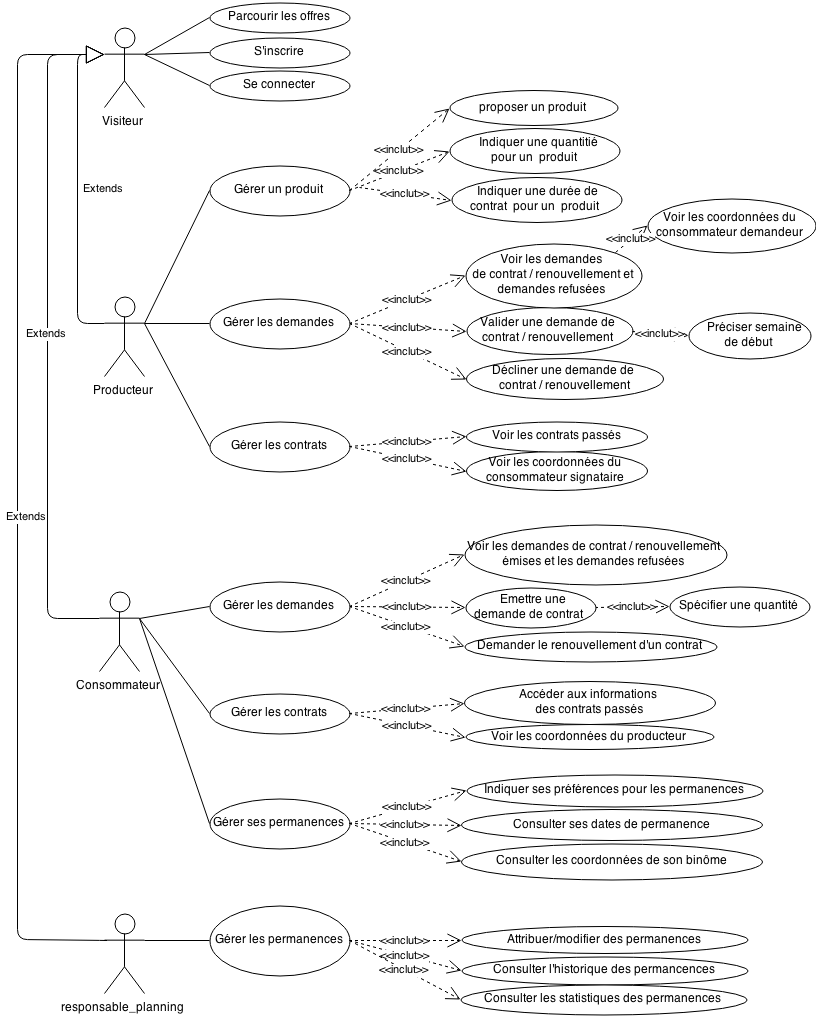
\includegraphics[height=1.35\textwidth]{./ressources/use_case.png}
\caption{Diagramme de cas d'utilisation.}
\end{figure}
\clearpage

\subsection{Description des cas d'utilisations et diagrammes de séquence système}

\subsubsection{Cas du visiteur :}
\begin{figure}[h]
\centering
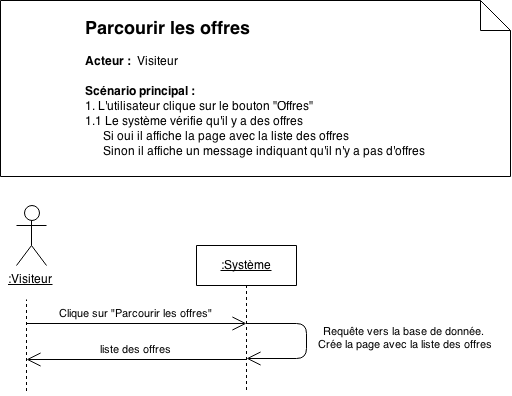
\includegraphics[width=.8\textwidth]{./ressources/desc_UC_parcourir_offres.png}
\caption{Description du cas "parcourir les offres"}
\end{figure}
\clearpage

\begin{figure}[!H]
\centering
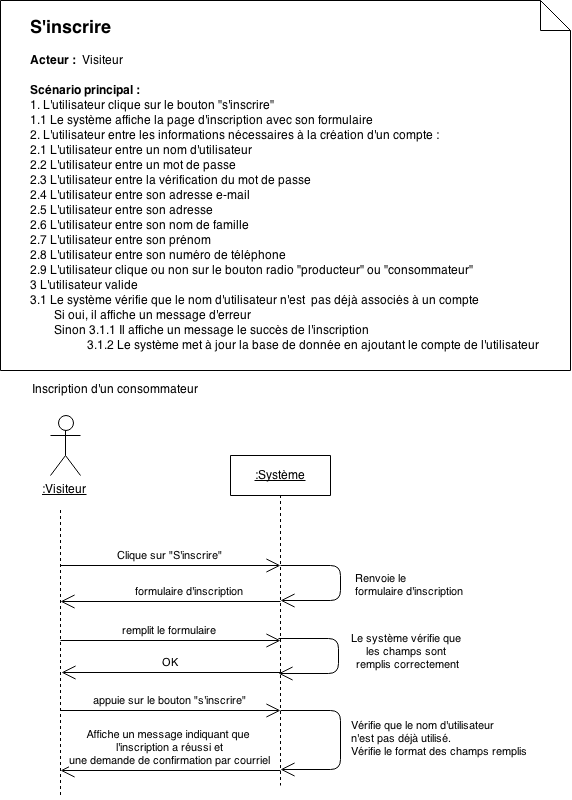
\includegraphics[width=1.\textwidth]{./ressources/desc_UC_inscrire.png}
\caption{Description du cas "s'inscrire"}
\end{figure}

\begin{figure}[!H]
\centering
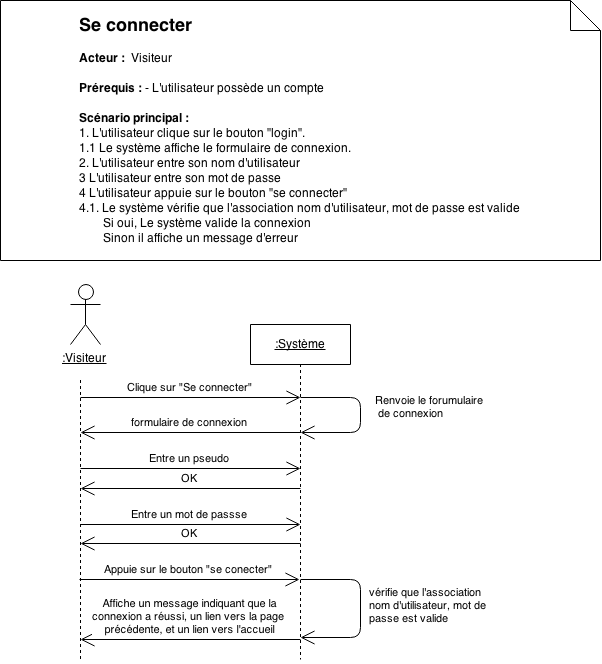
\includegraphics[width=1.\textwidth]{./ressources/desc_UC_connecter.png}
\caption{Description du cas "se connecter"}
\end{figure}
\clearpage

\subsubsection{Cas du producteur :}
\paragraph*{Gestion des produits :}
\begin{figure}[!Hb]
\centering
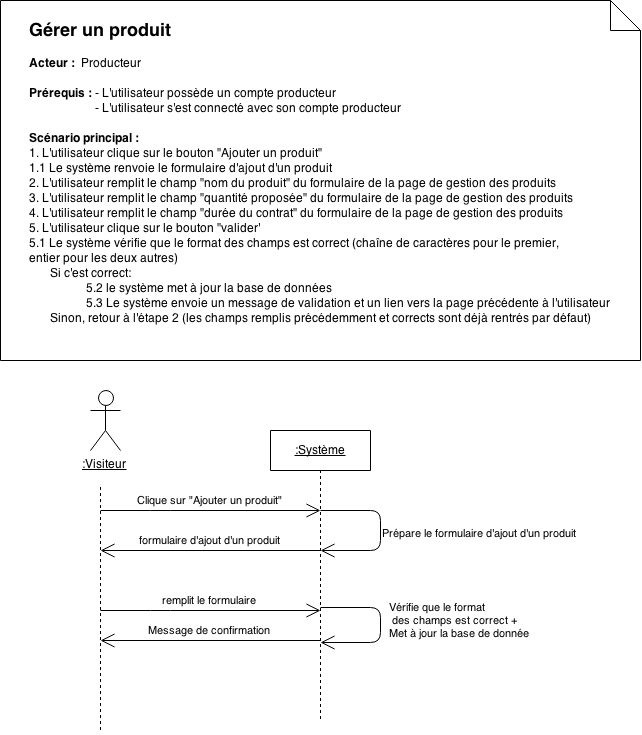
\includegraphics[width=1.\textwidth]{./ressources/desc_UC_gerer_produit.png}
\caption{Description du cas "gérer les produits"}
\end{figure}
\clearpage

\paragraph*{Gestion des demandes :}
\begin{figure}[!Hb]
\centering
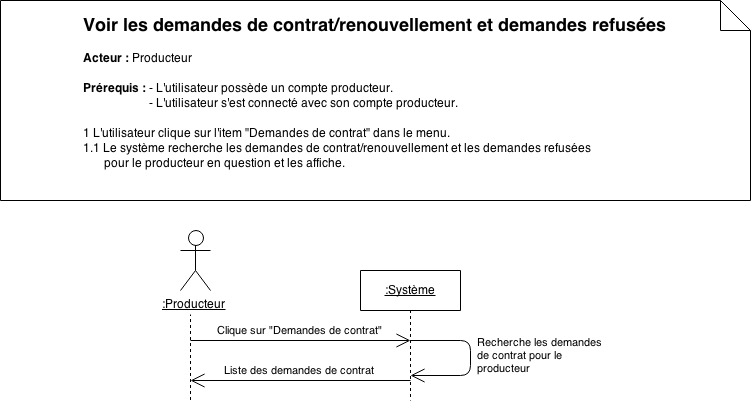
\includegraphics[width=1.1\textwidth]{./ressources/desc_UC_voir_demandes_prod.png}
\caption{Description du cas "Voir les demandes de contrats/renouvellement et demandes refusées (producteur)"}\vspace{80 mm}
\end{figure}
\clearpage

\begin{figure}[!H]
\centering
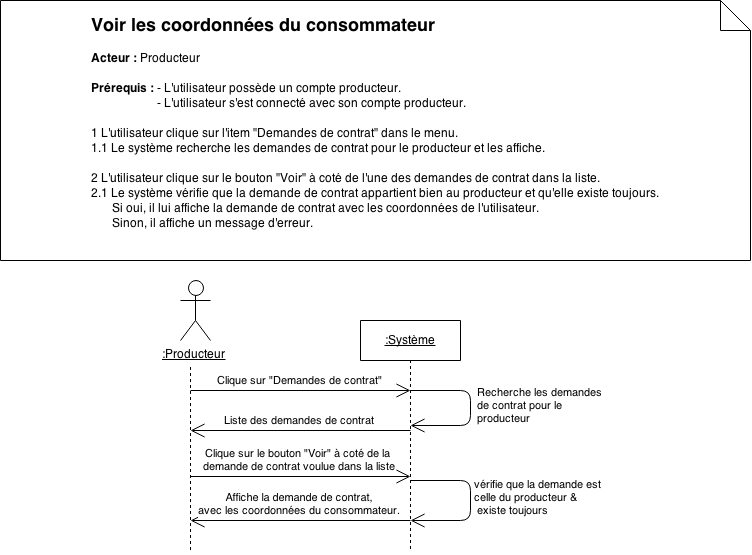
\includegraphics[width=1.\textwidth]{./ressources/desc_UC_coo_user.png}
\caption{Description du cas "Voir les coordonnées de l'utilisateur"}
\end{figure}
\clearpage

\begin{figure}[!H]
\centering
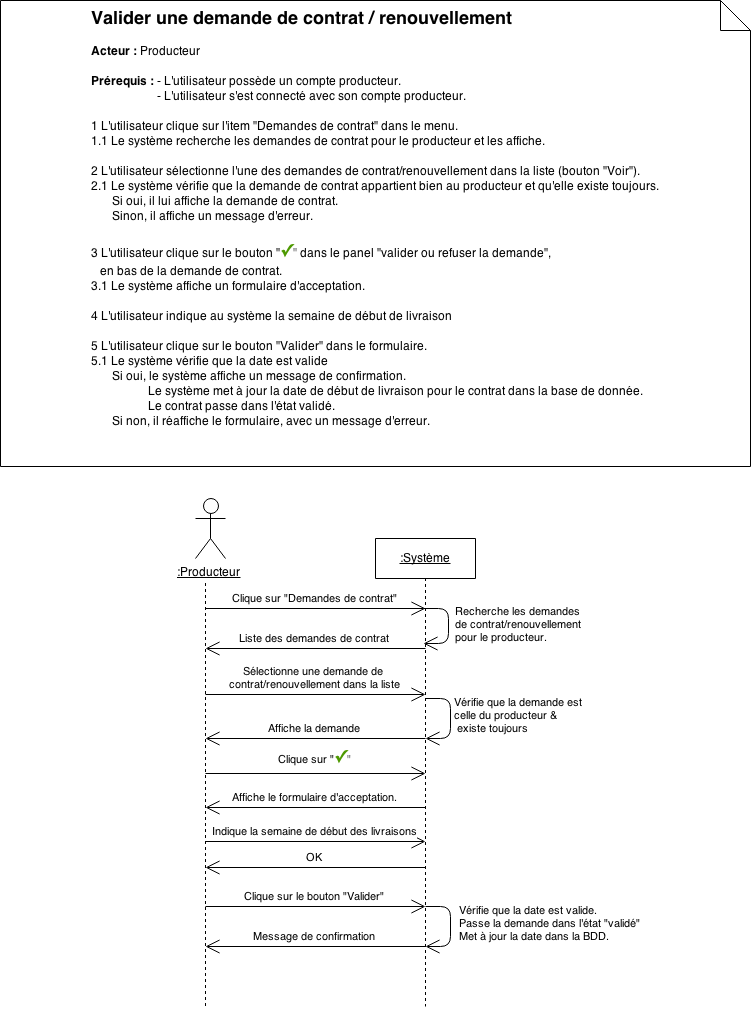
\includegraphics[width=1.\textwidth]{./ressources/desc_UC_valider_demande.png}
\caption{Description du cas "Valider une demande"}
\end{figure}
\clearpage

\begin{figure}[!H]
\centering
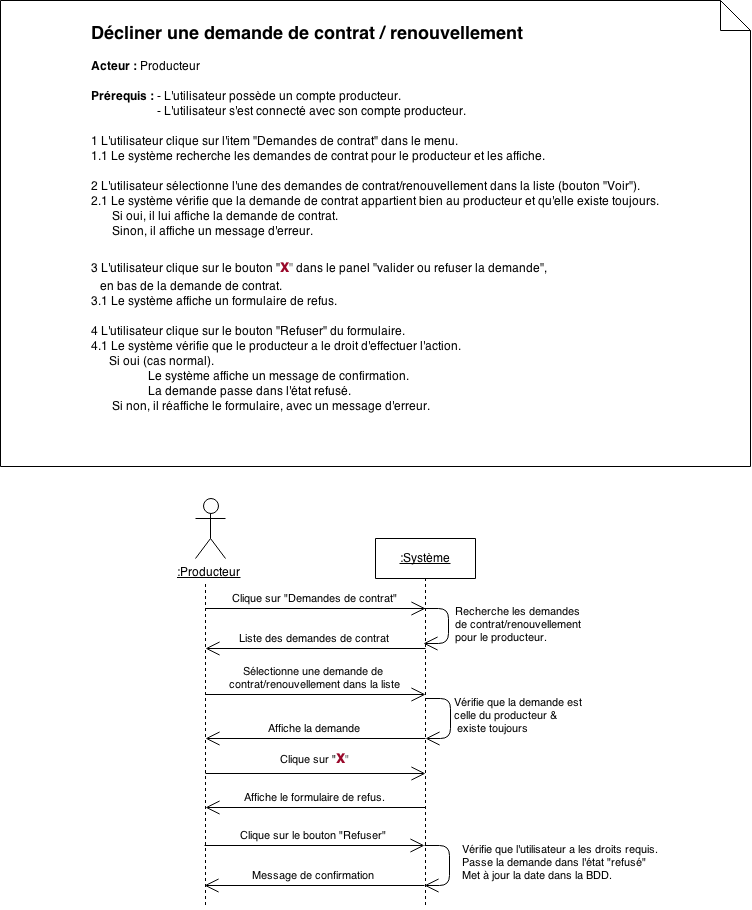
\includegraphics[width=1.\textwidth]{./ressources/desc_UC_decliner_demande.png}
\caption{Description du cas "Décliner une demande"}
\end{figure}
\clearpage

\paragraph*{Gestion des contrats :}

\begin{figure}[!H]
\centering
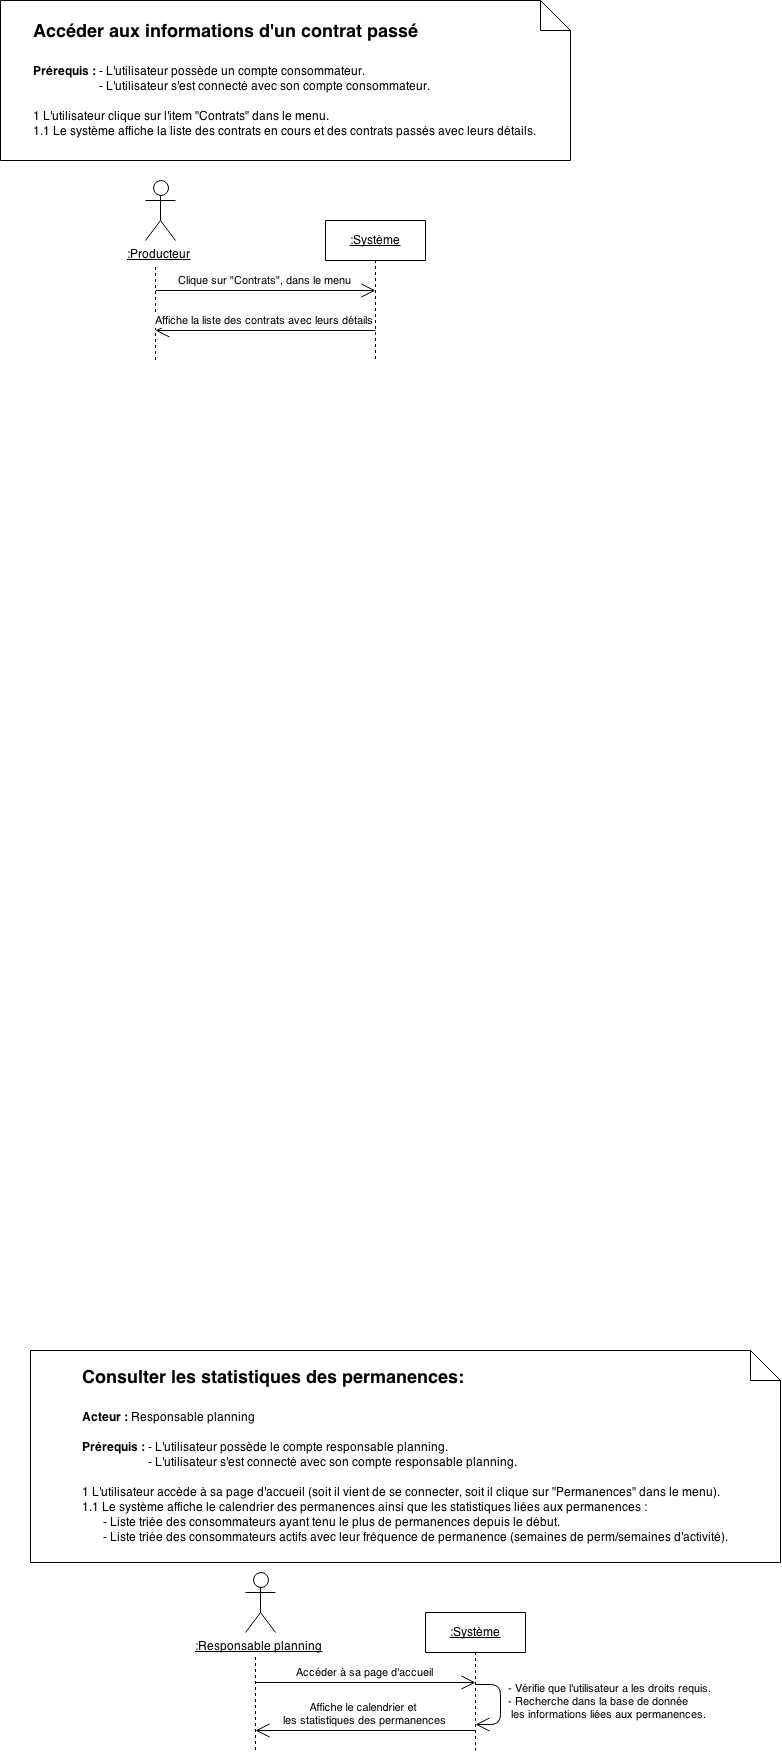
\includegraphics[width=1.\textwidth]{./ressources/desc_UC_contrats_passes.png}
\caption{Description du cas "Accéder aux informations des contrats passé (producteur)"}
\end{figure}
\clearpage

\begin{figure}[!H]
\centering
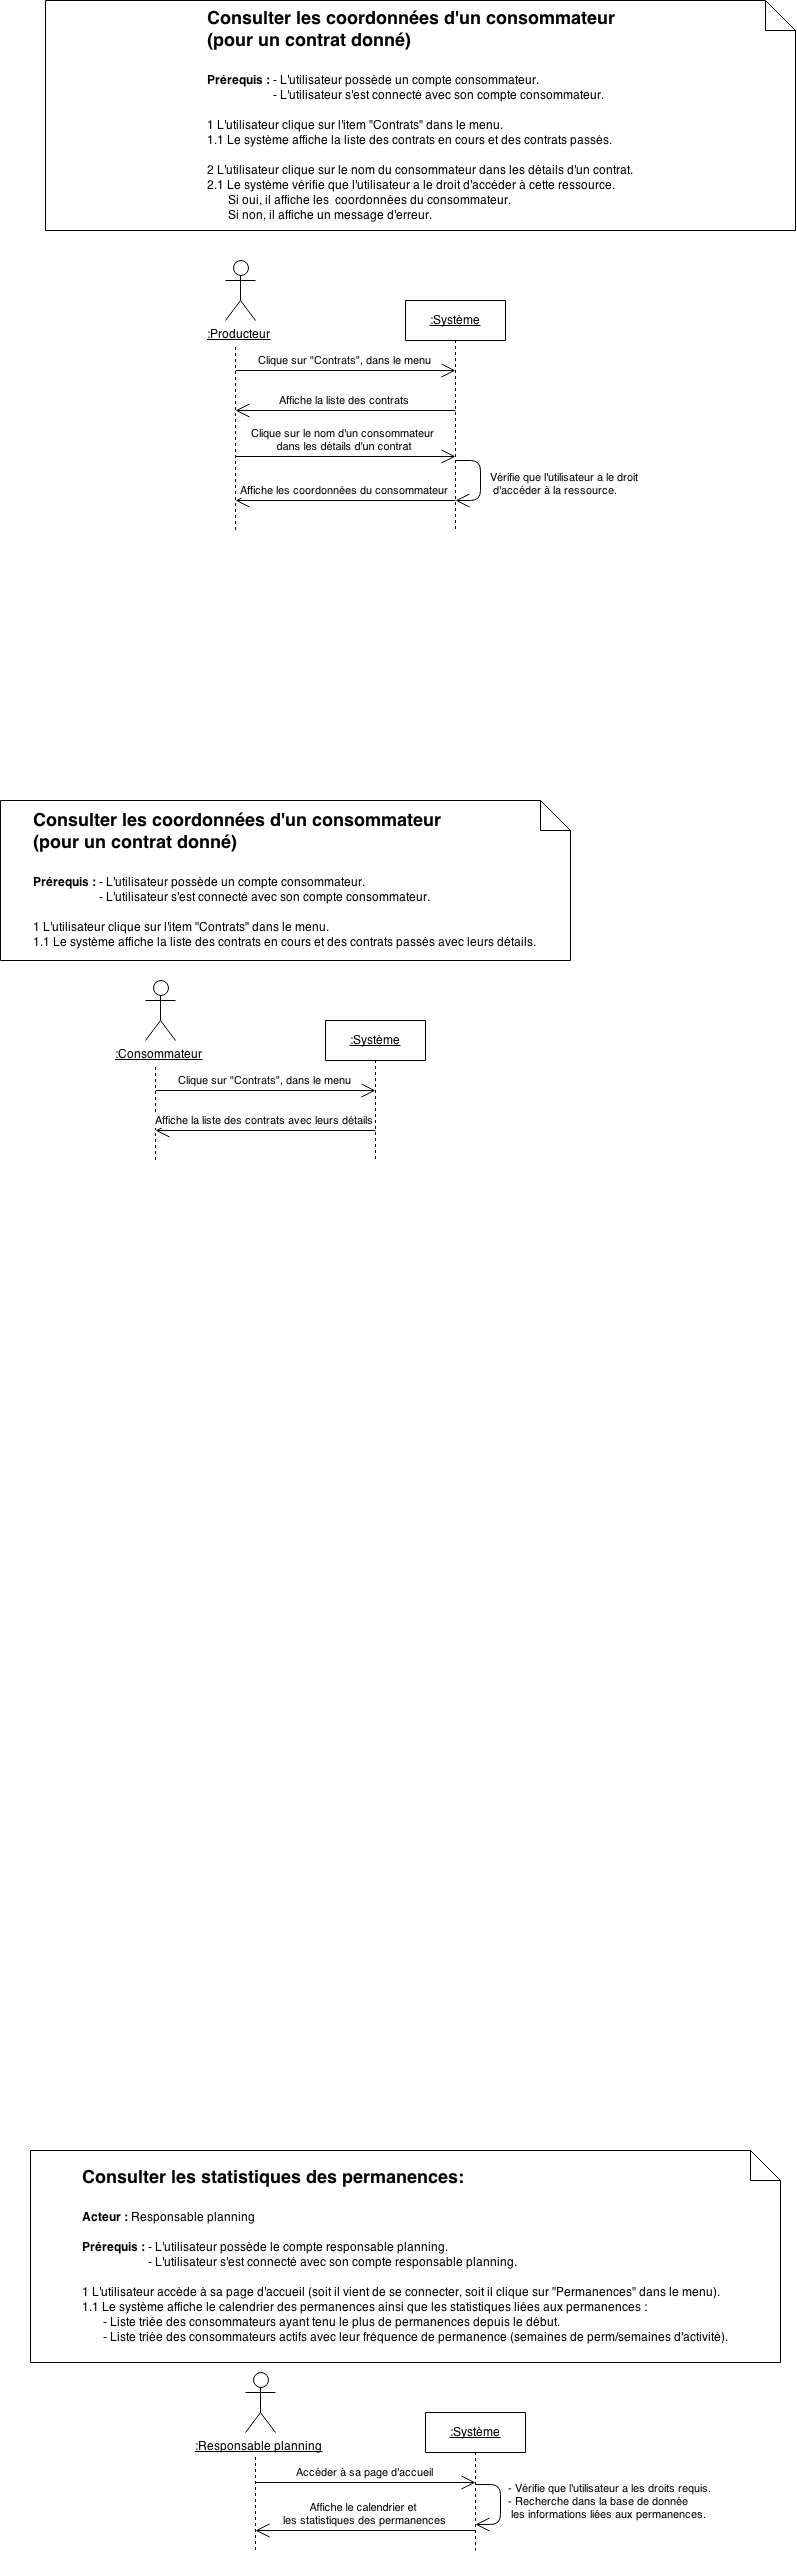
\includegraphics[width=1.\textwidth]{./ressources/desc_UC_coo_conso_contrats.png}
\caption{Description du cas "Consulter les coordonnées du consommateur signataire"}
\end{figure}
\clearpage



\subsubsection{Cas du consommateur :}
\paragraph*{Gestion des demandes :}

\begin{figure}[!H]
\centering
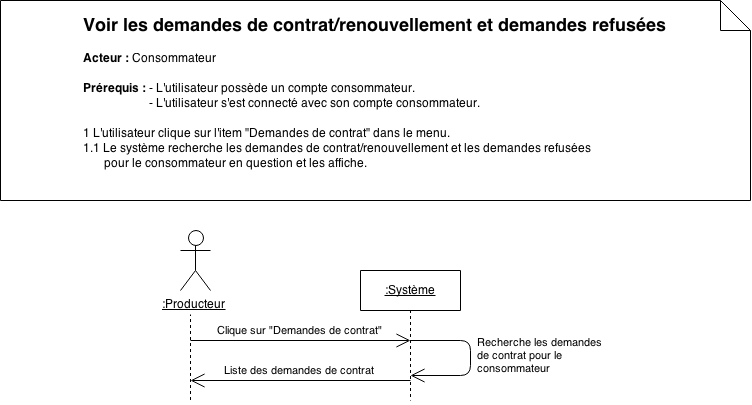
\includegraphics[width=1.\textwidth]{./ressources/desc_UC_voir_demandes_cons.png}
\caption{Description du cas "Voir les demandes de contrats/renouvellement et demandes refusées (consommateur)"}
\end{figure}
\clearpage

\begin{figure}[!H]
\centering
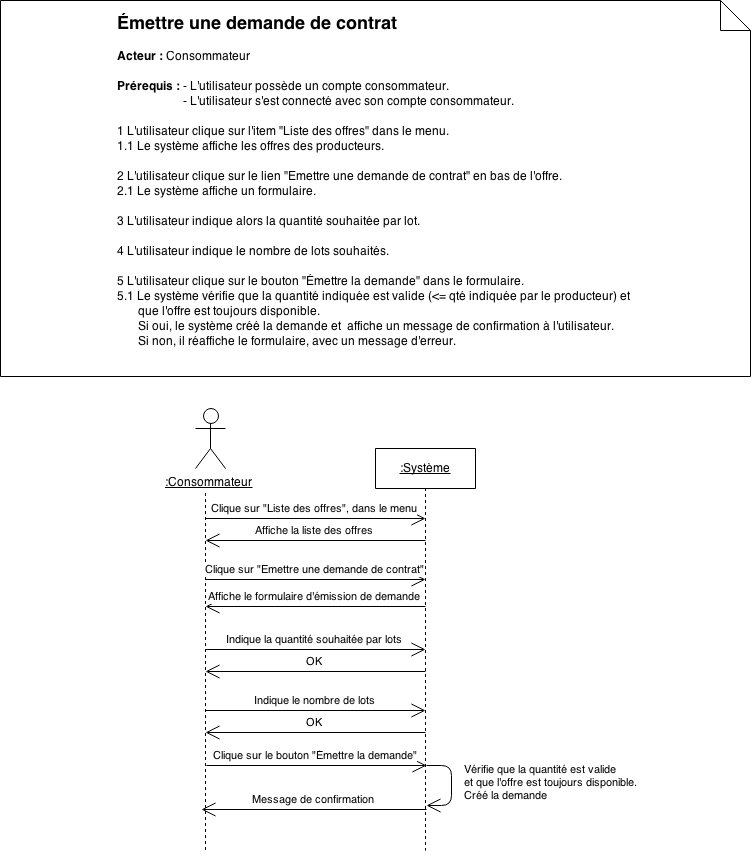
\includegraphics[width=1.\textwidth]{./ressources/desc_UC_emettre_demande.png}
\caption{Description du cas "Emettre une demande de contrat"}
\end{figure}
\clearpage

\begin{figure}[!H]
\centering
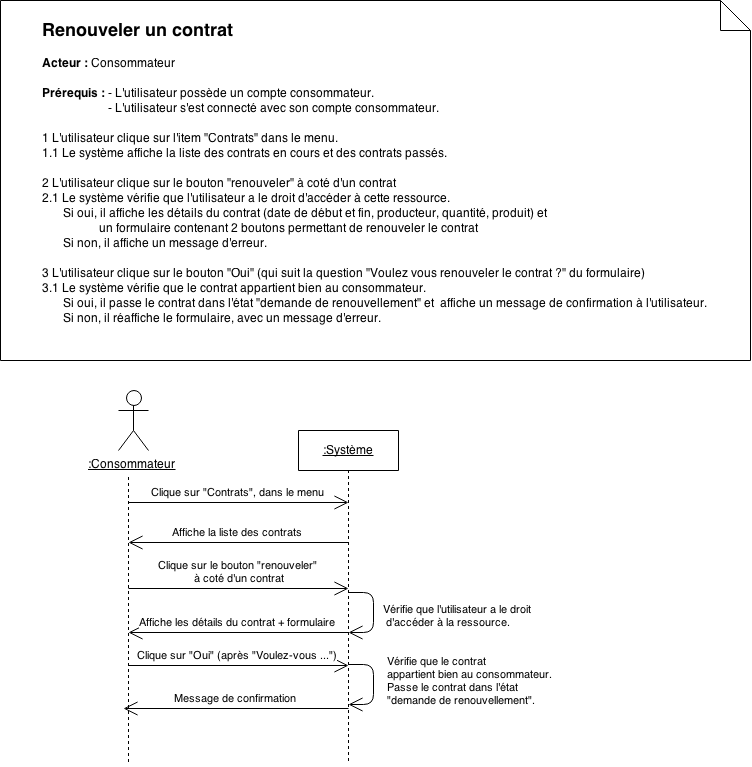
\includegraphics[width=1.\textwidth]{./ressources/desc_UC_demander_renouvellement.png}
\caption{Description du cas "Demander le renouvellement d'un contrat"}
\end{figure}
\clearpage

\paragraph*{Gestion des contrats :}
\begin{figure}[!Hb]
\centering
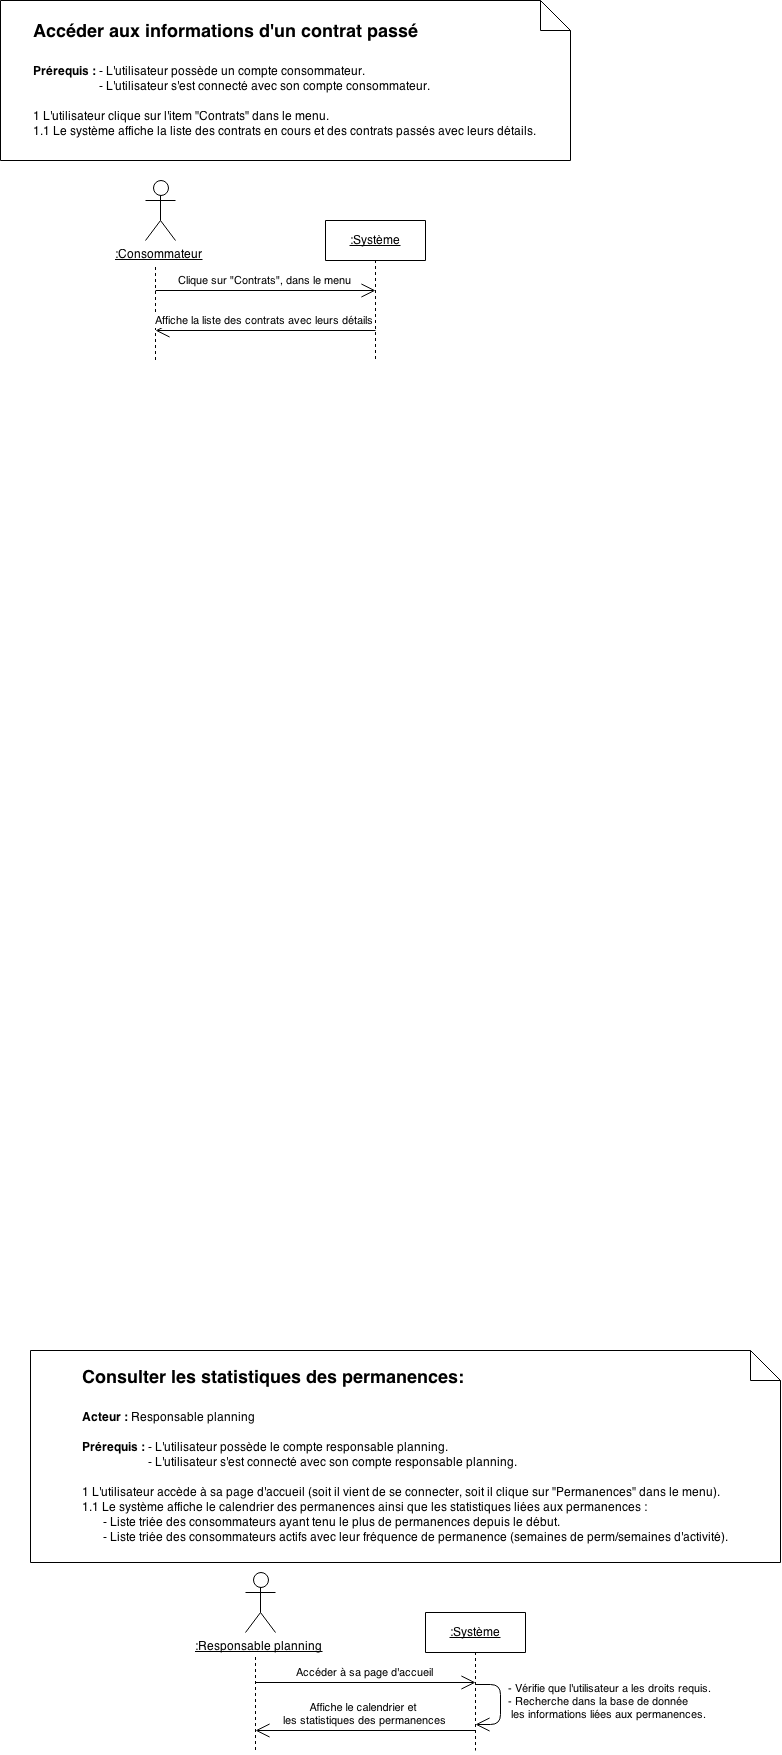
\includegraphics[width=.8\textwidth]{./ressources/desc_UC_contrats_passes_conso.png}
\caption{Description du cas "Accéder aux informations des contrats passés (consommateur)"}
\vspace{100mm}
\end{figure}
\clearpage

\begin{figure}[!H]
\centering
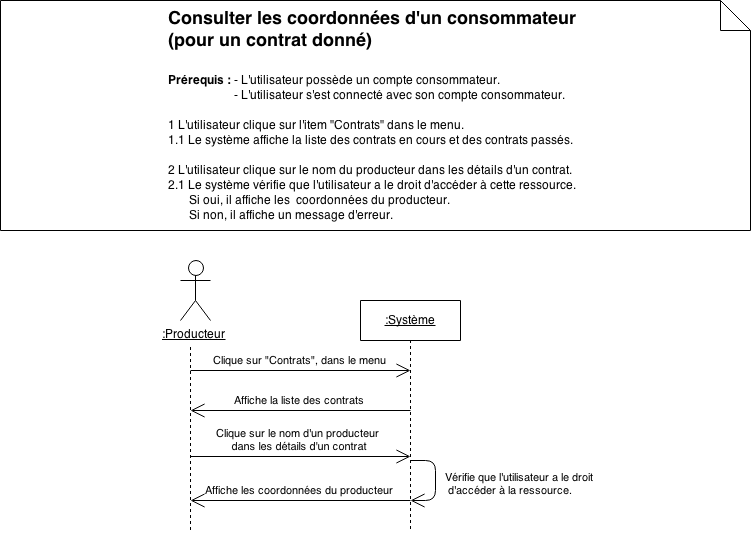
\includegraphics[width=1.1\textwidth]{./ressources/desc_UC_coo_prod_contrats.png}
\caption{Description du cas "Consulter les coordonnées d'un producteur"}
\end{figure}
\clearpage


\paragraph*{Gestion des permanences :}
\begin{figure}[!Hb]
\centering
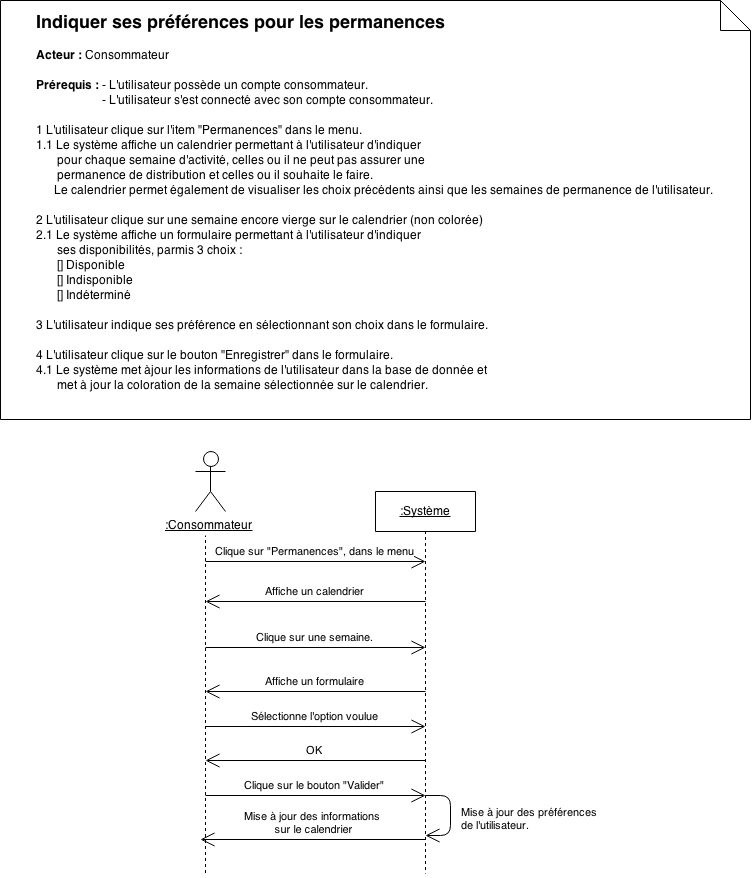
\includegraphics[width=1.\textwidth]{./ressources/desc_UC_preferences_calendrier.png}
\caption{Description du cas "Indiquer ses préférences concernant les permanences"}
\end{figure}
\clearpage

\begin{figure}[!H]
\centering
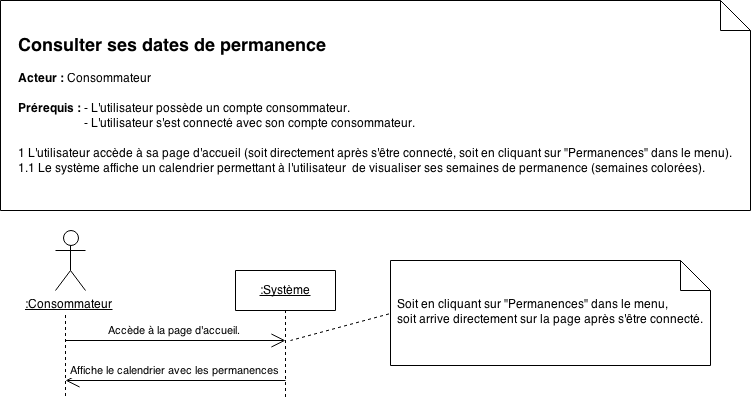
\includegraphics[width=1.\textwidth]{./ressources/desc_UC_consulter_permanences.png}
\caption{Description du cas "Consulter ses dates de permanence"}
\end{figure}
\clearpage

\begin{figure}[!H]
\centering
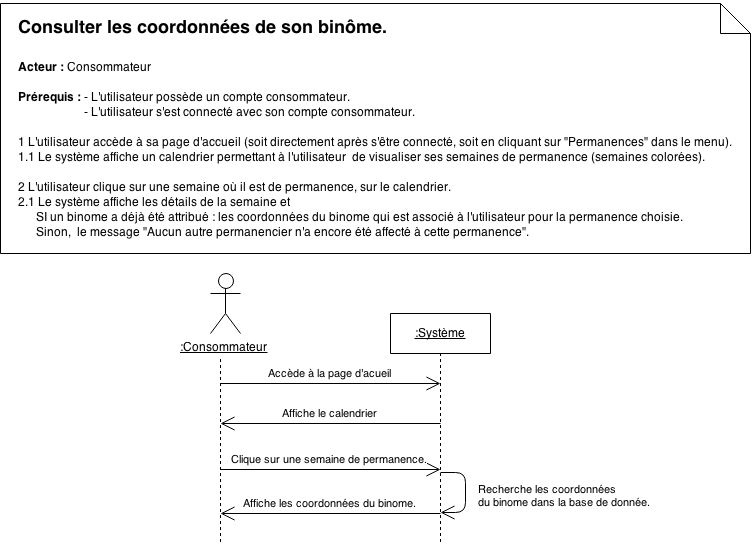
\includegraphics[width=1.\textwidth]{./ressources/desc_UC_coo_binome.png}
\caption{Description du cas "Consulter les coordonées de son binôme"}
\end{figure}
\clearpage

\subsubsection{Cas du responsable planning :}
\paragraph*{Gestion des permanences}
\begin{figure}[!Hb]
\centering
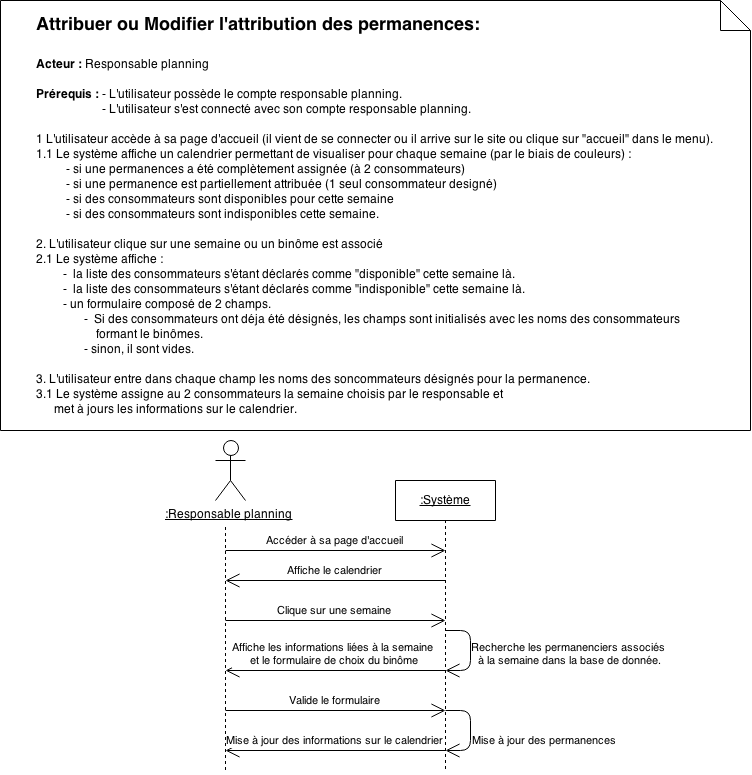
\includegraphics[width=1.\textwidth]{./ressources/desc_UC_attribuer_permanences.png}
\caption{Description du cas "Attribuer ou modifier l'attribution des permanences"}
\vspace{20mm}
\end{figure}
\clearpage

\begin{figure}[!H]
\centering
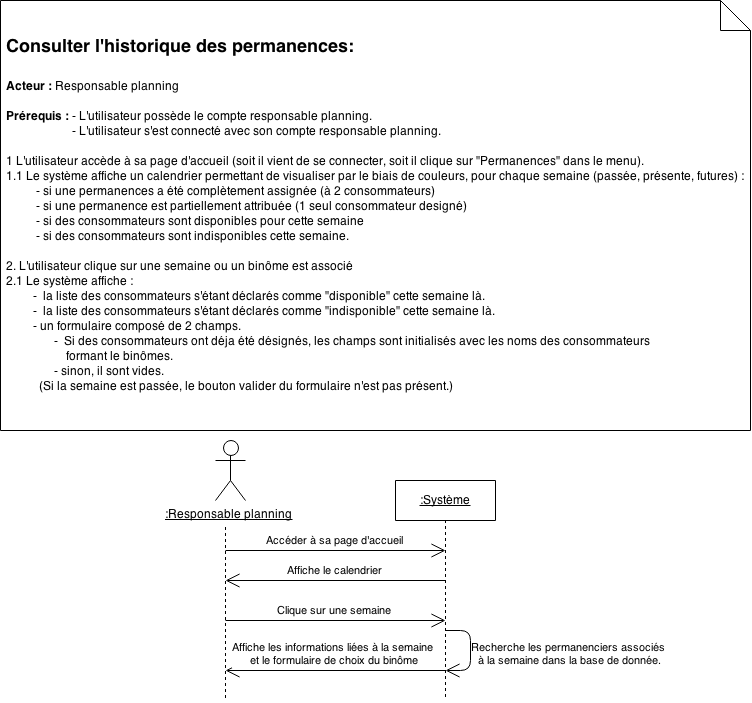
\includegraphics[width=1.\textwidth]{./ressources/desc_UC_voir_permanences.png}
\caption{Description du cas "Consulter l'historique des permanences"}
\end{figure}
\clearpage

\begin{figure}[!H]
\centering
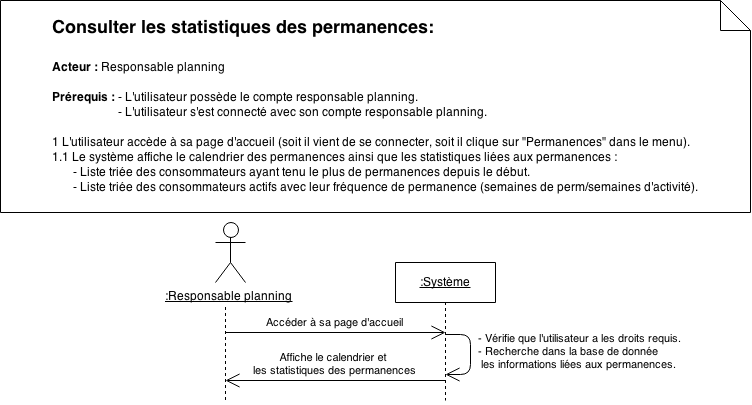
\includegraphics[width=1.\textwidth]{./ressources/desc_UC_stats_permanences.png}
\caption{Description du cas "Consulter les statistiques des permanences"}
\end{figure}
\clearpage



\subsection{Diagramme de classes d'analyse}
\begin{figure}[!Hb]
\centering
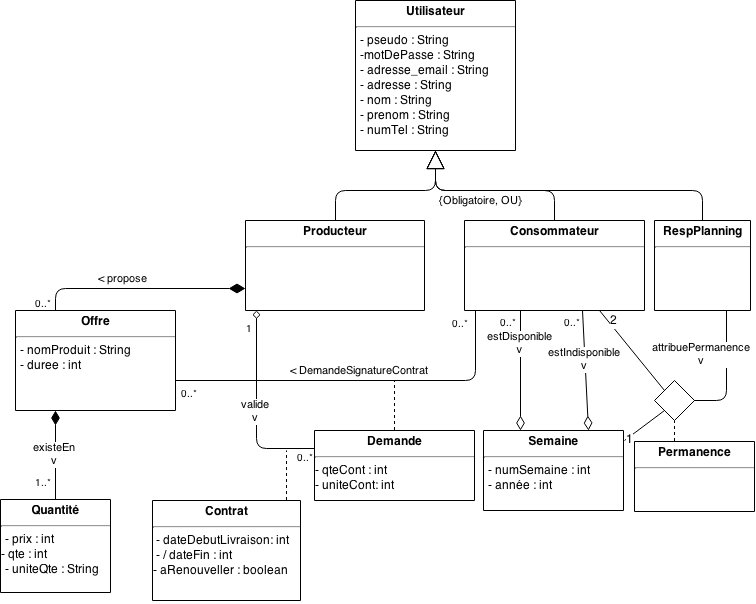
\includegraphics[height=.9\textwidth]{./ressources/class_analyse.png}
\caption{Diagramme de classes d'analyse.}
\vspace{50mm}
\end{figure}
\clearpage

% ------------------------------------------------------------------------------
% --------------------------- CONCEPTION ---------------------------------------
% ------------------------------------------------------------------------------

\section{Conception}

\begin{figure}[!hp]
\centering
\subsection{Architecture générale~~~~~~~~~~~~~~~~~~~~~~~~~~~~~~~}
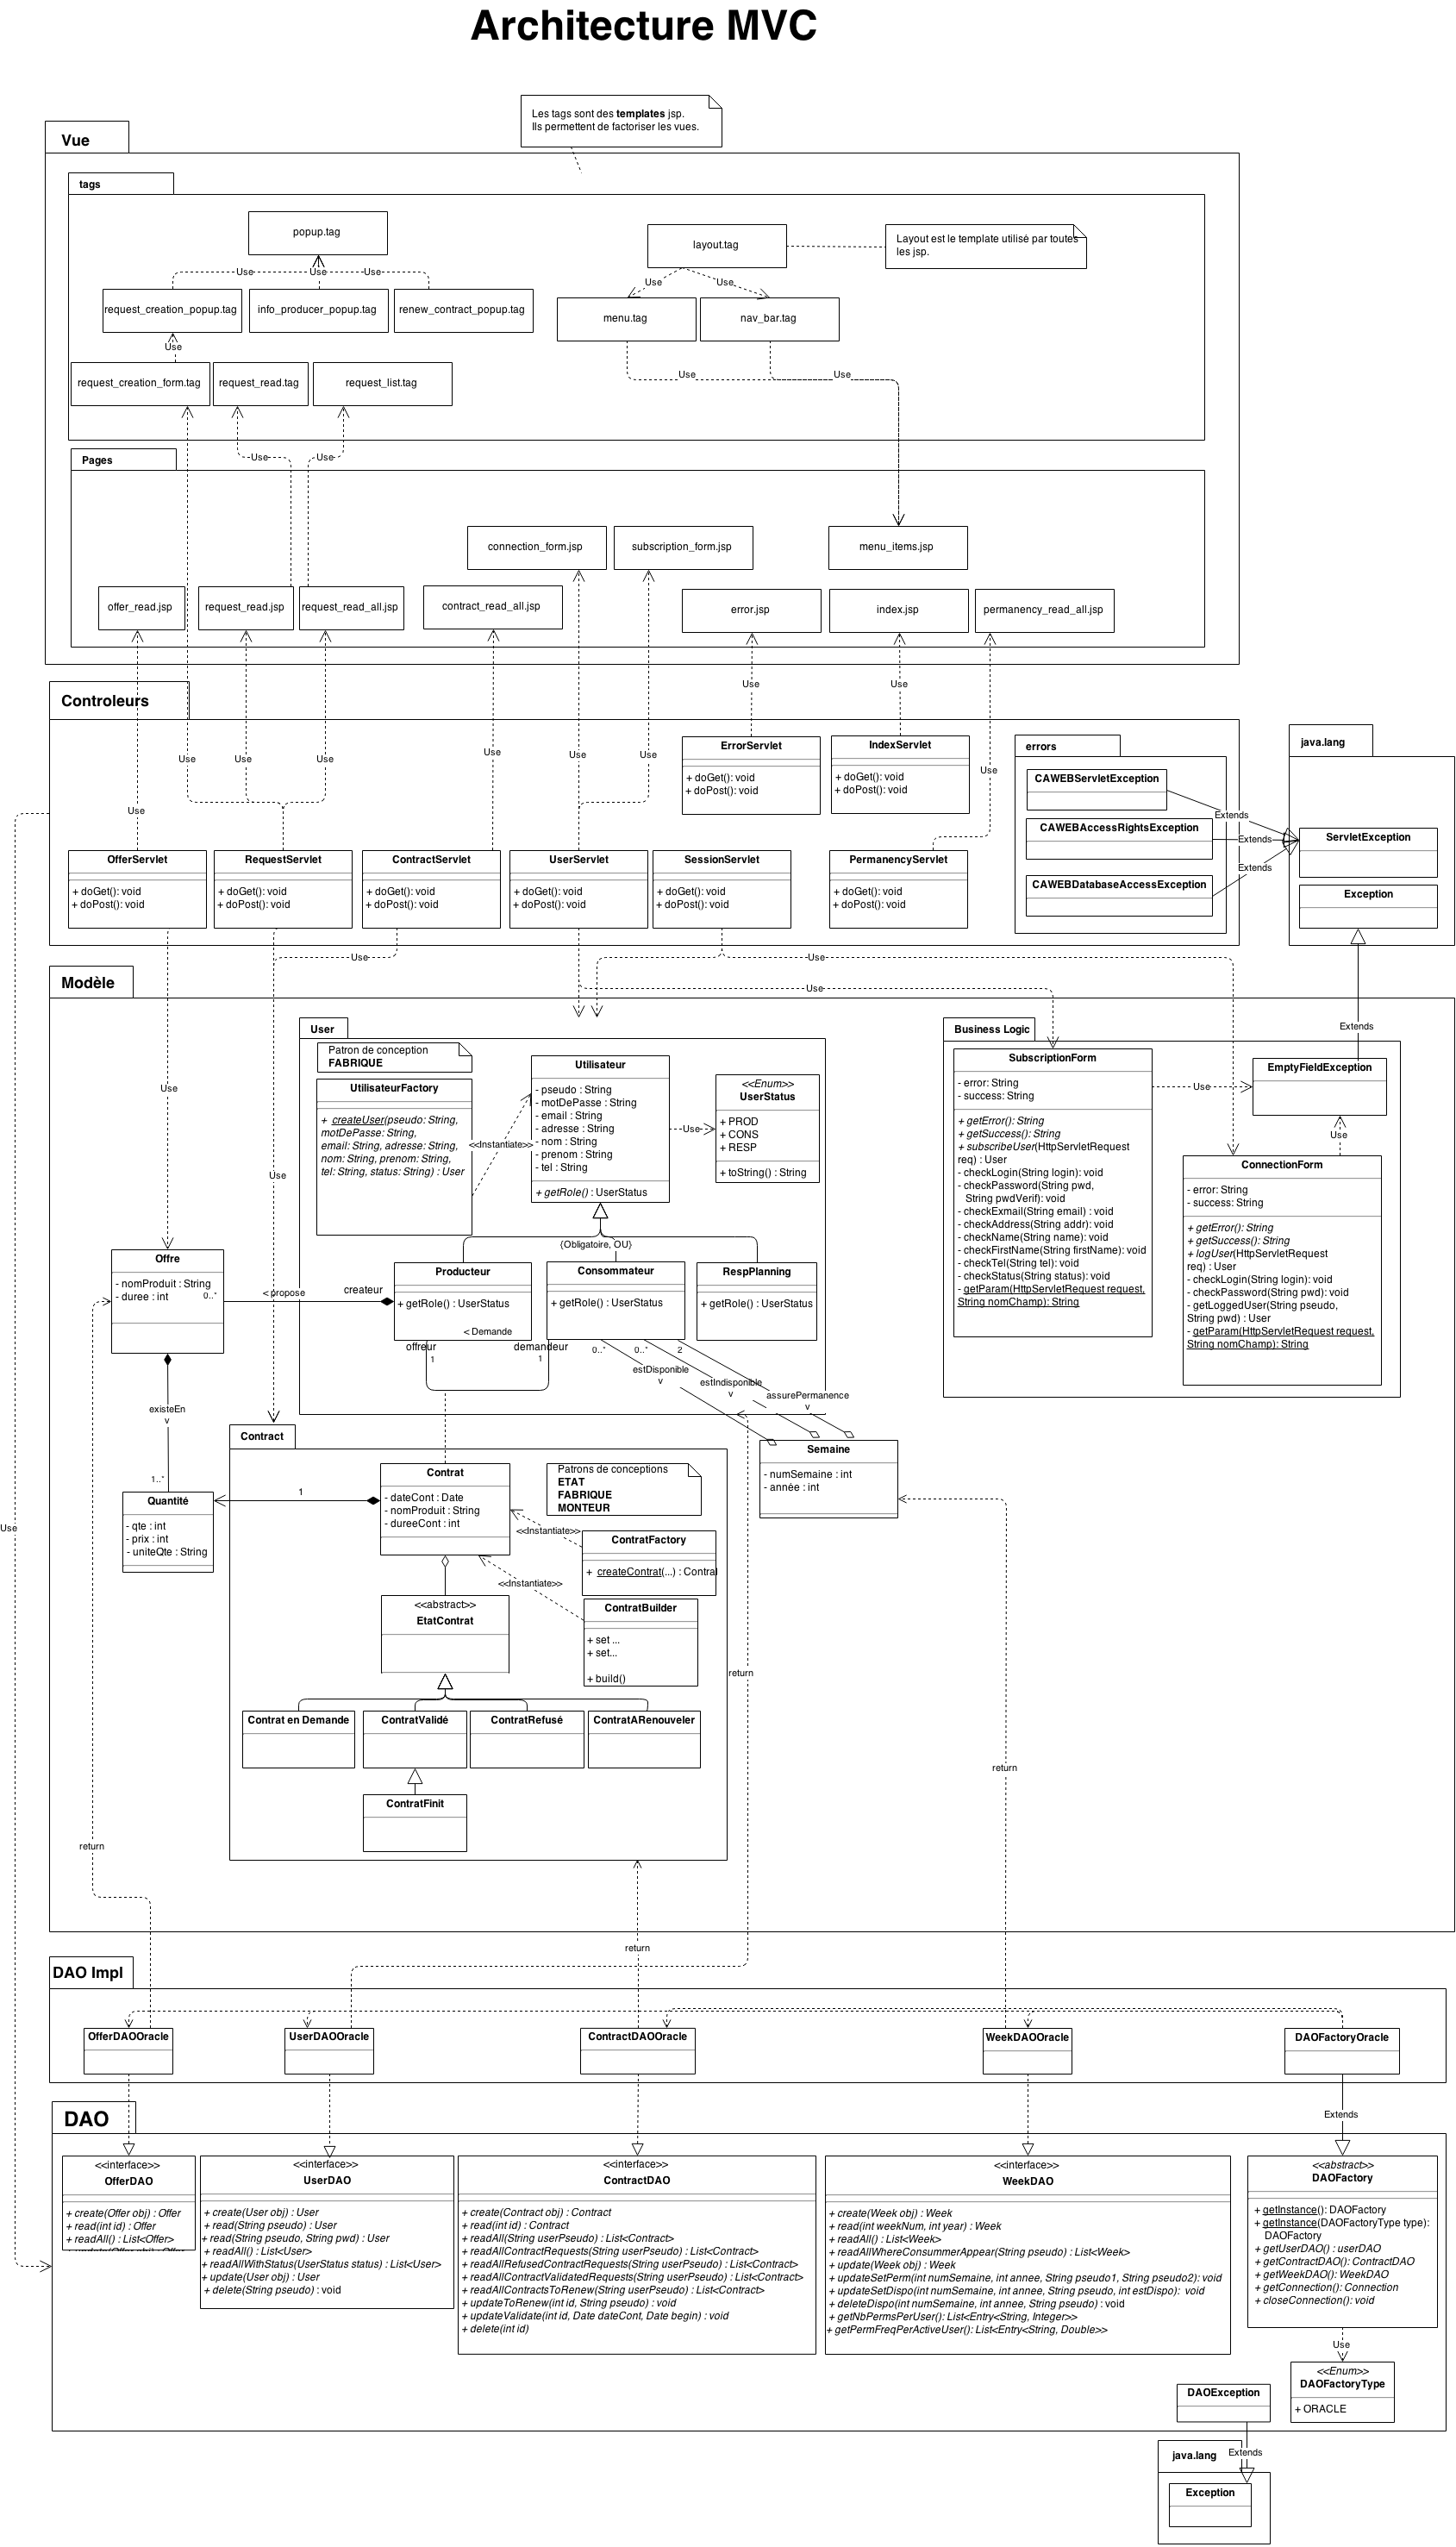
\includegraphics[height=1.1\textwidth]{./ressources/architecture.png}
\caption{Architecture logicielle.}
\end{figure}
\clearpage


\begin{figure}[!hp]
\centering
\subsection{Diagramme de classes logicielles~~~~~~~~~~~~~~~~~~~~~~~~~~~~~~~}
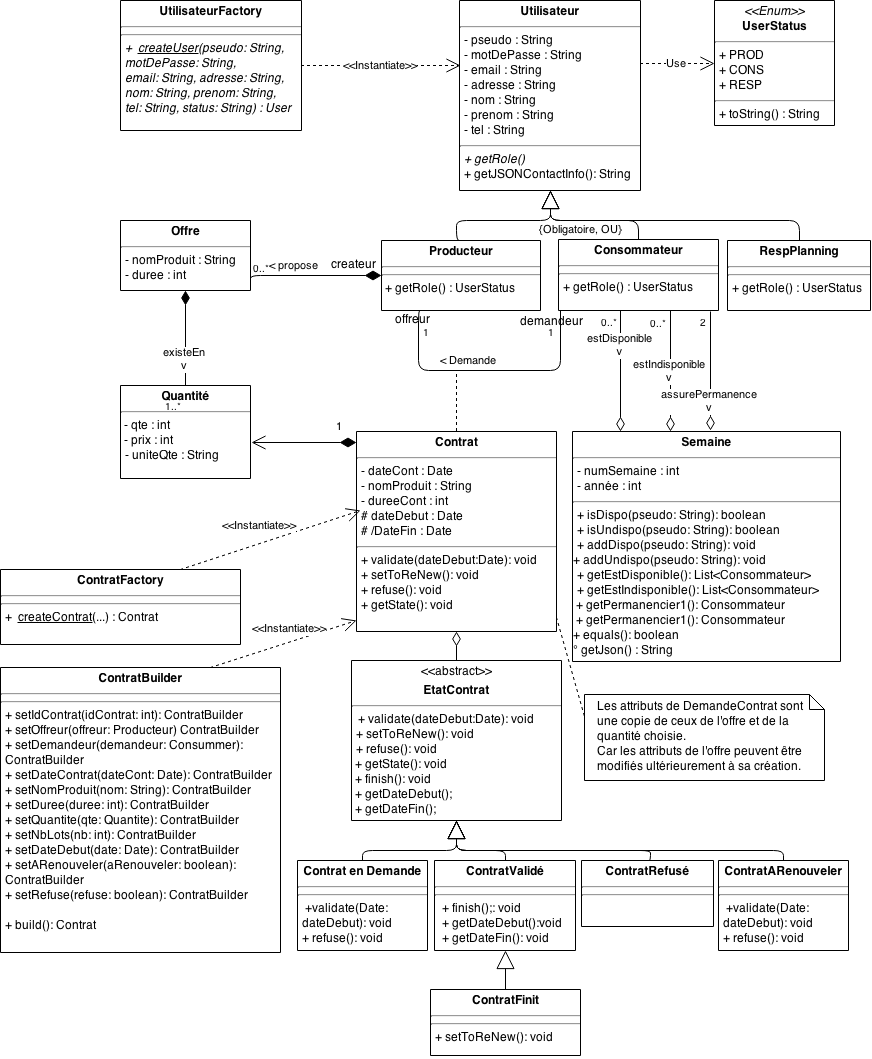
\includegraphics[height=1.\textwidth]{./ressources/class_logicielle.png}
\caption{Diagramme de classes logicielle.}
\end{figure}
\clearpage

\subsection{Diagrammes de séquence}
\begin{figure}[!hp]
\centering
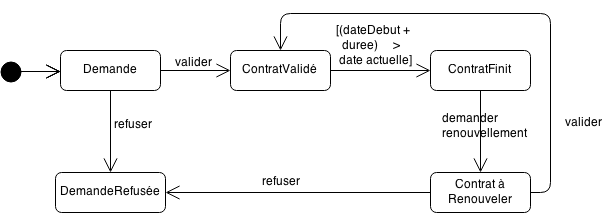
\includegraphics[width=1.\textwidth]{./ressources/etat_transition_contrat.png}
\caption{Cycle de vie d'un contrat}
\end{figure}
\clearpage

\subsection{Diagrammes d'états-transitions}
\begin{figure}[!hp]
\centering
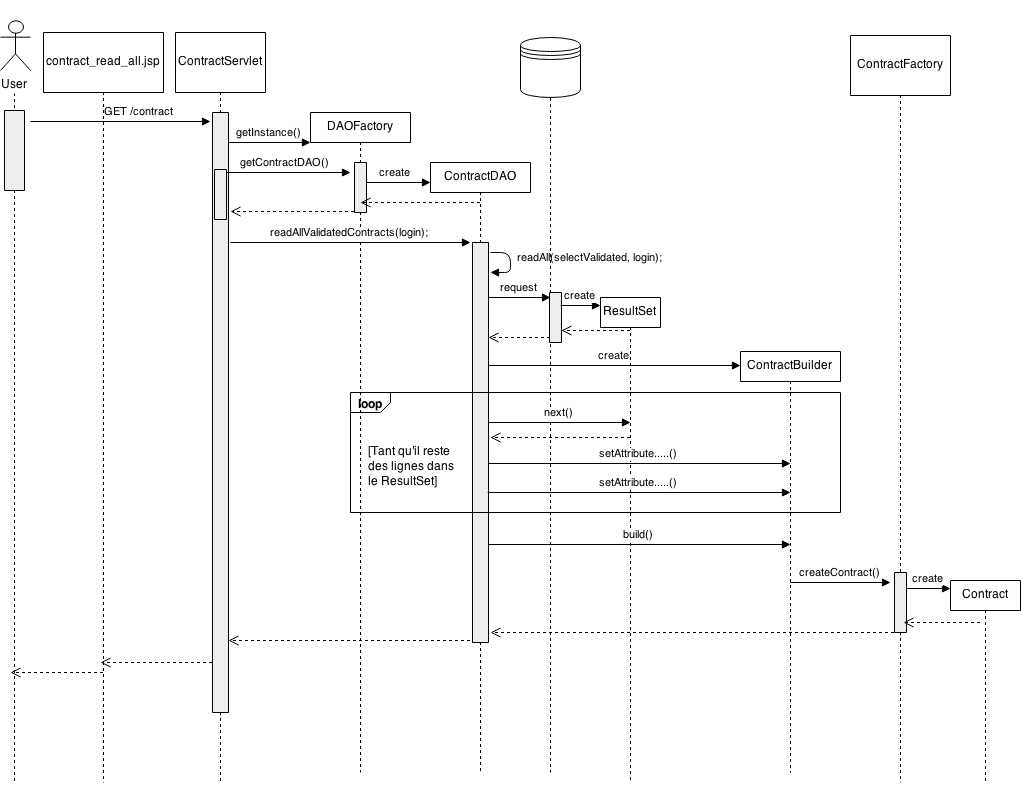
\includegraphics[width=1.\textwidth]{./ressources/seq_contrats.png}
\caption{Diagramme de séquence pour la lecture de la liste des contrats}
\end{figure}
\clearpage
Nous n'avons mis qu'un seul schéma pour illustrer la séquence des appels, car cette séquence ne varie que trés peu en fonction des requêtes.\\
Dans tous les cas, les mêmes actions ont lieu :
\begin{itemize}
\item Une servlet reçoit une requête HTTP de la part du client.
\item La servlet traite les informations passées en paramètres.
\item La servlet fait appel à un DAO.
\item Le DAO effectue des requêtes vers la base de donnée puis stock les informations sous formes d'objets du modèle.
\item La servlet récupère les objets ainsi créés et effectue les traitements nécessaires avec.
\item La servlet transmet les informations à la vue, et l'appelle.
\end{itemize}

\clearpage
\section{Manuel Utilisateur}

\subsection{Pour le visiteur}
\paragraph{S'inscrire}
L'utilisateur peut s'inscrire en tant que consommateur ou producteur en saisissant les informations requises dans le formulaire d'inscription.
Le formulaire est accessible par un simple clique sur "Inscription" en haut de la page d'accueil.

\paragraph{Se connecter}
Pour s'inscrire, cliquer sur le lien "Login" en haut de la page d'accueil, puis remplir le formulaire.

\paragraph{Voir la liste des offres}
La liste des offres est consultable par tous les utilisateurs (inscris ou non), via le lien "Liste des offres" du menu.

\subsection{Pour le producteur}
\paragraph{Gestion des produits}
Le producteur peut voir la liste de ses produits proposés en cliquant sur "Offres proposées".\\
Il peut également proposer de nouvelles offres en cliquant sur "Créer une offre" dans le menu.\\
Enfin, il peut voir l'ensemble des offres proposées par les producteurs, en cliquant sur l'onglet "Liste des offres" dans le menu.

\paragraph{Gestion des demandes}
Par le biais de l'onglet "Demandes de contrats" du menu, le producteur a accés aux demandes de contrats, ainsi qu'aux demandes de renouvellement émises par les consommateurs.\\
Sur cette même page, il peut également avoir accés au demandes qu'il a refusé.\\
En cliquant sur l'une des demandes de contrat / renouvellement, l'utilisateur peut accéder aux détails de la demande (coordonnées de l'utilisateur et précisions sur l'offre) et ensuite l'accepter ou la refuser.

\paragraph{Gestion des contrats}
Le producteur peut voir les contrats qu'il a passé en cliquant sur l'onglet "Contrats" du menu.\\
Il peut ensuite accéder aux coordonnées du signataire du contrats en cliquant sur son nom.

\subsection{Pour le consommateur}
\paragraph{Gestion des demandes}
L'utilisateur peut créer une demande en allant dans "Liste des Offres", puis en cliquant sur "Emettre une demande" au bas de l'une des offres.\\
L'utilisateur peut consulter les demandes qu'il a émises dans l'onglet "Demandes de contrats" du menu. Il a ainsi accés à ses demandes de contrats, demandes de renouvellement et à ses demandes qui ont été refusées.\\
Pour chaque demande, il peut voir le détail de celle-ci en cliquant sur "voir" à coté de la demande.

\paragraph{Gestion des contrats}
En cliquant sur l'onglet "Offres" du menu, le consommateur peut voir ses contrats en cours et ses contrats terminés. \\
A coté de la description de chaque contrat se trouve le nom du producteur associé. En cliquant sur le nom du producteur, le consommateur peut accéder à ses coordonnées.\\

A coté des contrats terminés se trouve le lien "Renouveler" permettant à l'utilisateur de faire une demande de renouvellement pour le contrat.

\paragraph{Gestion des permanences}
Dans l'onglet permanence, le consommateur trouvera un calendrier lui permettant de consulter les préférences qu'il a déjà indiquées pour chaque semaine, ainsi que les permanences qui lui sont attribuées.\\
En cliquant sur une semaine, il peut changer ses préférences. \\
Dans le cas où une permanence lui a été attribuée, le consommateur peut également voir les coordonnées de son binome, en cliquant sur la semaine de permanence.

\subsection{Pour le responsable du planning}
\paragraph{Gestion des permanences}
L'onglet "Permanences", qui se trouve également être la page d'accueil, permet de voir et modifier les permanences des consommateurs.\\
Par le biais du calendrier, le responsable peut accéder aux informations des semaines passées, présentes et futures (permanences et disponibilités des consommateurs).\\
En cliquant sur une semaine en particulier, il peut voir les consommateurs et producteurs disponibles et indisponibles cette semaine; et il peut modifier ou attribuer des permanences.\\

Enfin, sur cette même page se trouvent des statistiques sur les permanences.

\subsection{Note sur l'accessibilité}
L'application web propose un design responsive, capable de s'adapter aux différents appareils de l'utilisateur (smartphones, tablettes, ordinateurs, télévisions).\\
Par exemple, le menu latéral présent sur les grands écrans, laisse place à un menu déroulant sur tablettes et smartphones.\\
De la même manière, le reste du contenu s'adapte en taille pour permettre la meilleure visibilité possible quelque soit le périphérique utilisé.

\begin{figure}[h]
\centering
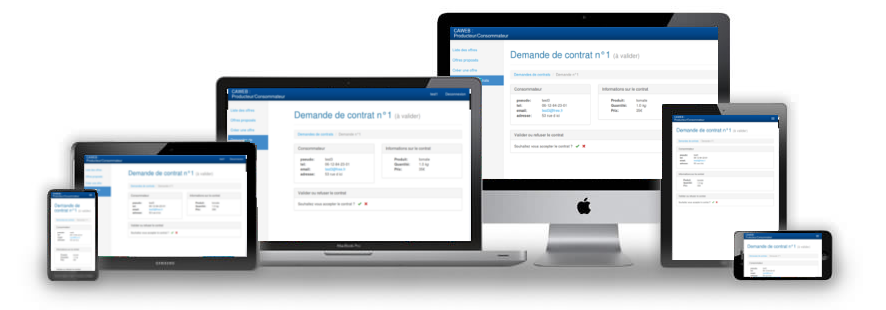
\includegraphics[width=1.\textwidth]{./ressources/responsive_design.png}
\caption{Illustration du design responsive de l'application.}
\end{figure}

\clearpage
\section{Bilan sur les outils de modélisation}
Afin de réaliser nos différents diagrammes, nous avons utilisé l'application web \textit{Draw.io Pro} \footnote{Draw.io : \url{www.draw.io}}.\\
Nous n'avons pas rencontré de difficulté particulière à ce niveau. Les formes "UML" et "SysML" disponibles dans \textit{Draw.io} permettent de réaliser l'ensemble des diagrammes de la norme UML2.


\end{document}